\small
%\begin{itemize}
%    \item \textbf{Read and write waveform data in various formats} (MiniSEED, SAC, GSE, SEG Y, \dots) with a unified interface.
%    \item \textbf{Database and web service access clients} for the new FDSN web services, NERIES, IRIS DMC, ArcLink, SeisHub and Earthworm (experimental).
%    \item \textbf{Many seismological signal processing routines} like filters, trigger, instrument correction, array analysis, beamforming, \dots
%    \item \textbf{Support for inventory data} (SEED, XSEED, RESP, and StationXML support)
%    \item \textbf{Event data handling} (Supports the latest QuakeML 1.2 version)
%    \item \textbf{Unified time handling} Uses UTC $\Rightarrow$ No ambiguities
%\end{itemize}
%
%\begin{center}
%    +
%\end{center}
%
%\begin{center}
%    \textbf{The full power and flexibility of Python.}
%\end{center}
\section*{What Can I Do with ObsPy?}
\begin{multicols}{2}
Easy to use helper functions to access local files and online data centers give
\textbf{quick access to all data neccessary for seismological data analysis}.

All acquired information is exposed to
the user in \textbf{ObsPy's core classes that handle waveform data, station and event
metadata in a unified, consistent fashion, regardless of the data source}. This makes it easy to
combine data from different sources in unified workflows, both interactively and
automated.

ObsPy's core classes have many convenience routines for signal processing
directly attached for \textbf{quick, reproducible and well tested execution of
common processing tasks}.
\columnbreak
\begin{center}
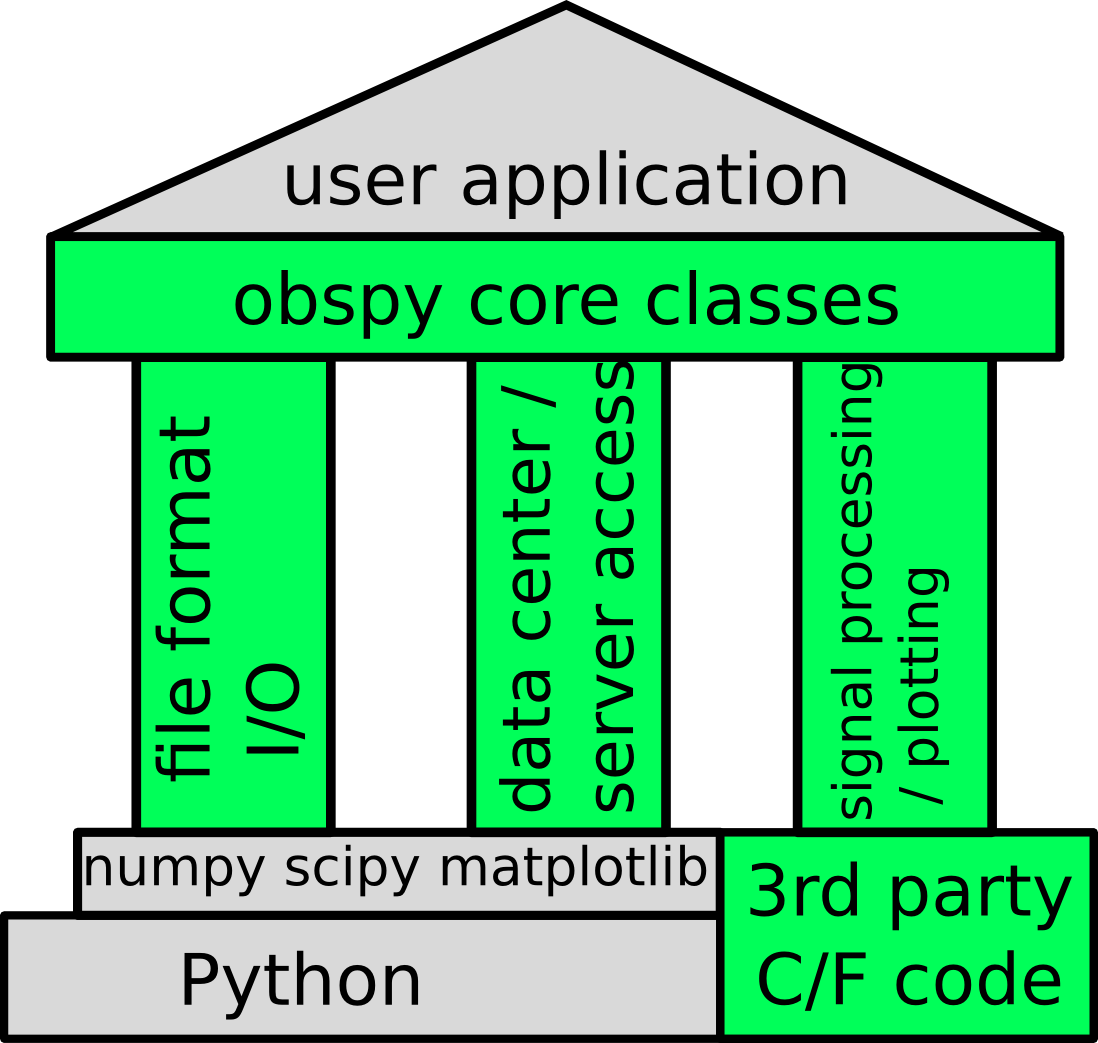
\includegraphics[width=0.65\columnwidth]{./images/obspy_pillars.png} \\
\end{center}
\end{multicols}
\vspace{\MyBoxVSep}

\begin{center}
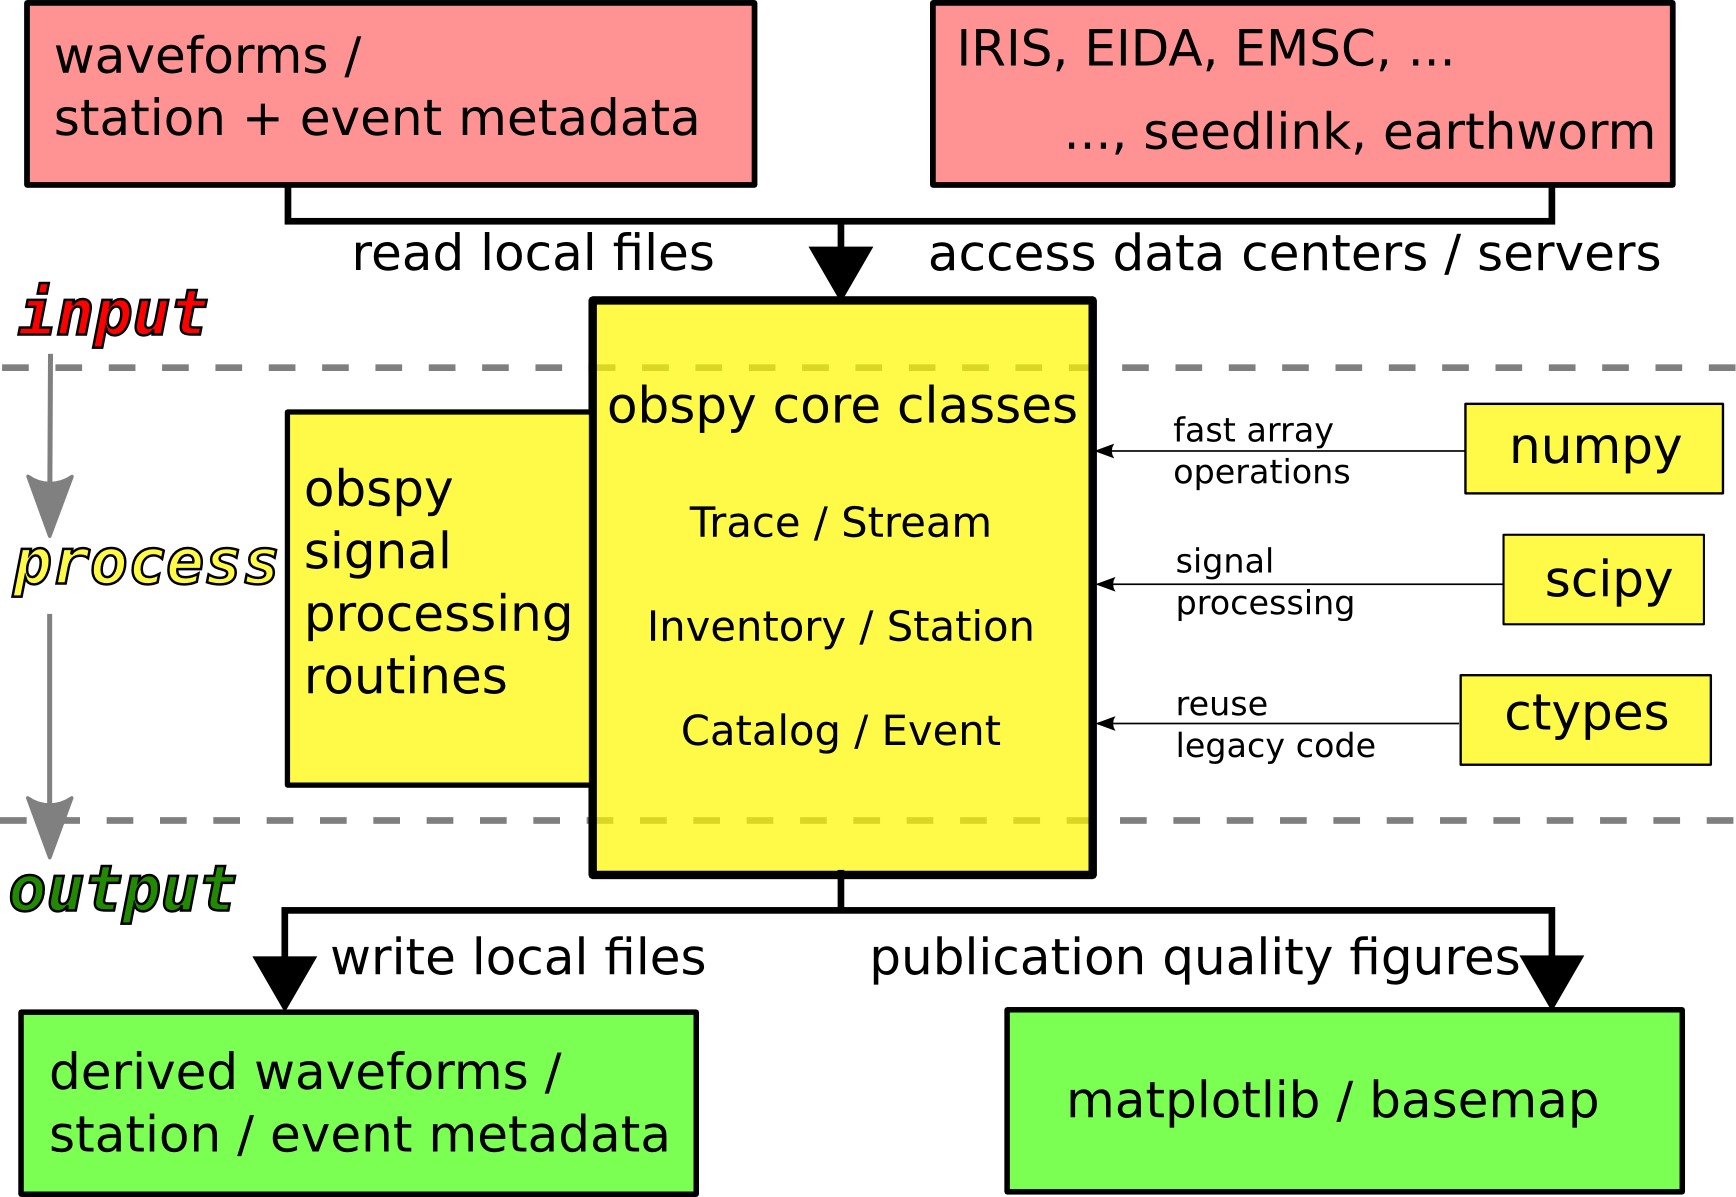
\includegraphics[width=0.764\columnwidth]{./images/obspy_workflow.png} \\
\end{center}
